\chapter{在Direct3D中绘制2(Drawing in Direct3D Part 2)}
\begin{flushleft}
本章介绍我们将在本书其余部分使用的一些绘图模式。 本章首先介绍一种绘图优化的方法,我们将其称为“帧资源”。使用帧资源,我们修改渲染循环,这样我们就不必每帧刷新命令队列; 这提高了CPU和GPU的利用率。 接下来,我们介绍渲染项的概念,并解释我们如何根据更新频率划分常量数据。 此外,我们更详细地检查根签名,并了解其他根参数类型:根描述符和根常量。 最后,我们展示了如何绘制一些更复杂的对象; 到本章结束时,您将能够绘制类似丘陵和山谷,圆柱体,球体和动画波浪模拟的表面。\\
~\\
{\large Objectives:}
\begin{itemize}
    \item 了解对渲染过程的修改,不要求我们每帧刷新命令队列,从而提高性能。
    \item 了解其他两种类型的根签名参数类型:根描述符和根常量。
    \item 探索如何在程序上生成和绘制常见的几何形状,如网格,圆柱体和球体。
    \item 了解我们如何在CPU上设置顶点动画并使用动态顶点缓冲区将新顶点位置上传到GPU。
\end{itemize}
\end{flushleft}

%---- 7.1 ------
\section{帧资源(Frame Resources)}
\begin{flushleft}
回忆 4.2 节,CPU和GPU并行工作。 CPU构建并提交命令列表(除了其他CPU工作之外),GPU处理命令队列中的命令。 目标是让CPU和GPU忙碌,以充分利用系统上可用的硬件资源。 到目前为止,在我们的演示中,我们已经每帧同步CPU和GPU一次。 两个例子解释这种同步的必要性:\\
\begin{itemize}
    \item 1.在GPU完成执行命令之前,不能重置命令分配器(command allocator)。 假设我们没有进行同步,以便CPU在GPU处理完当前帧n之前可以继续下一帧n + 1:如果CPU在帧n + 1中重置命令分配器,但GPU仍在处理命令 从第n帧开始,我们将清除GPU仍在使用的命令。
    \item 2.在GPU完成执行引用常量缓冲区的绘图命令之前,CPU无法更新常量缓冲区。 此示例对应于4.2.2节和图4.7中描述的情况。 假设我们没有进行同步,以便CPU在GPU完成处理当前帧n之前可以继续下一帧n + 1:如果CPU在帧n + 1中覆盖常量缓冲区数据,但GPU还没有 执行引用帧n中的常量缓冲区的绘制调用,然后常量缓冲区包含当GPU执行帧n的绘制调用时的错误数据。
\end{itemize}
因此,我们一直在每帧结束时调用 D3DApp::FlushCommandQueue,以确保GPU已完成执行帧的所有命令。 此解决方案有效,但由于以下原因效率低下:\\
\begin{itemize}
    \item 1.在帧开始时,GPU将不会有任何要处理的命令,因为我们等待清空命令队列。 它必须等到CPU构建并提交一些命令才能执行。
    \item 2.在帧结束时,CPU正在等待GPU完成处理命令。
\end{itemize}
所以每一帧,CPU和GPU都会在某些时候空闲。\\
~\\
该问题的一个解决方案是创建CPU修改每个帧所需的资源的循环数组。 我们称这种资源为帧资源,我们通常使用三个帧资源元素的循环数组。 对于帧n,CPU将循环通过帧资源队列以获得下一个可用(即,未被GPU使用)帧资源。 然后,CPU将执行任何资源更新,并在GPU处理先前帧时构建和提交帧n的命令列表。 然后CPU继续进行第n + 1帧并重复。 如果帧资源阵列有三个元素,这可以使CPU在GPU之前达到两帧,从而确保GPU保持忙碌状态。 下面是我们在本章中用于“Shapes”演示的帧资源类的示例。 由于CPU只需要在此演示中修改常量缓冲区,因此帧资源类仅包含常量缓冲区。\\
\end{flushleft}
\begin{lstlisting}
// Stores the resources needed for the CPU to build
// the command lists
// for a frame. The contents here will vary from app
// to app based on
// the needed resources.
struct FrameResource
{
public:
    FrameResource(ID3D12Device* device, UINT passCount, UINT objectCount);
    FrameResource(const FrameResource& rhs) = delete;
    FrameResource& operator=(const FrameResource& rhs) = delete;
    ~FrameResource();
    // We cannot reset the allocator until the GPU is
    // done processing the
    // commands. So each frame needs their own
    // allocator.
    Microsoft::WRL::ComPtr<ID3D12CommandAllocator> CmdListAlloc;
    
    // We cannot update a cbuffer until the GPU is done
    // processing the
    // commands that reference it. So each frame needs
    // their own cbuffers.
    std::unique_ptr<UploadBuffer<PassConstants>> PassCB = nullptr;
    std::unique_ptr<UploadBuffer<ObjectConstants>>
    ObjectCB = nullptr;
    // Fence value to mark commands up to this fence
    // point. This lets us
    // check if these frame resources are still in use
    // by the GPU.
    UINT64 Fence = 0;
};

FrameResource::FrameResource(ID3D12Device* device,
                             UINT passCount, UINT
                             objectCount)
{
    ThrowIfFailed(device->CreateCommandAllocator(
        D3D12_COMMAND_LIST_TYPE_DIRECT,
        IID_PPV_ARGS(CmdListAlloc.GetAddressOf())));
    PassCB = std::make_unique<UploadBuffer<PassConstants>>(
        device,
        passCount, 
        true);
    ObjectCB = std::make_unique<UploadBuffer<ObjectConstants>>(
        device,
        objectCount, true);
}
FrameResource::˜FrameResource() {}
\end{lstlisting}
\begin{flushleft}
然后,我们的应用程序类将三个帧资源的向量实例化,并设置成员变量以跟踪当前帧资源:\\
\end{flushleft}
\begin{lstlisting}
static const int NumFrameResources = 3;
std::vector<std::unique_ptr<FrameResource>> mFrameResources;
FrameResource* mCurrFrameResource = nullptr;
int mCurrFrameResourceIndex = 0;
void ShapesApp::BuildFrameResources()
{
    for(int i = 0; i < gNumFrameResources; ++i)
    {
        mFrameResources.push_back(std::make_unique<FrameResource>(
                                      md3dDevice.Get(), 
                                      1, 
                                      (UINT)mAllRitems.size()));
    }
}
\end{lstlisting}
\begin{flushleft}
现在,对于CPU帧n,算法的工作原理如下:\\
\end{flushleft}
\begin{lstlisting}
void ShapesApp::Update(const GameTimer& gt)
{
    // Cycle through the circular frame resource array.
    mCurrFrameResourceIndex = (mCurrFrameResourceIndex + 1) % NumFrameResources;
    mCurrFrameResource = mFrameResources[mCurrFrameResourceIndex];
    // Has the GPU finished processing the commands of
    // the current frame
    // resource. If not, wait until the GPU has
    // completed commands up to
    // this fence point.
    if(mCurrFrameResource->Fence != 0 &&
       mCommandQueue->GetLastCompletedFence() < mCurrFrameResource->Fence)
    {
        HANDLE eventHandle = CreateEventEx(nullptr, false, 
                                  false, EVENT_ALL_ACCESS);
        ThrowIfFailed(mCommandQueue->SetEventOnFenceCompletion(
             mCurrFrameResource->Fence, eventHandle));
        WaitForSingleObject(eventHandle, INFINITE);
        CloseHandle(eventHandle);
    }
    // […] Update resources in mCurrFrameResource (like cbuffers).
}
void ShapesApp::Draw(const GameTimer& gt)
{
    // […] Build and submit command lists for this frame.
    // Advance the fence value to mark commands up to
    // this fence point.
    mCurrFrameResource->Fence = ++mCurrentFence;
    // Add an instruction to the command queue to set a
    // new fence point.
    // Because we are on the GPU timeline, the new fence
    // point won’t be
    // set until the GPU finishes processing all the
    // commands prior to
    // this Signal().
    mCommandQueue->Signal(mFence.Get(), mCurrentFence);
    // Note that GPU could still be working on commands
    // from previous
    // frames, but that is okay, because we are not
    // touching any frame
    // resources associated with those frames.
}
\end{lstlisting}
\begin{flushleft}
请注意,此解决方案不会阻止等待。 如果一个处理器处理帧的速度比另一个处理器快得多,那么一个处理器最终将不得不等待另一个处理器赶上,因为我们不能让一个处理器远远超过另一个处理器。 如果GPU处理命令的速度比CPU提交工作的速度快,那么GPU将处于空闲状态。 一般来说,如果我们试图推动图形限制,我们希望避免这种情况,因为我们没有充分利用GPU。 另一方面,如果CPU总是以比GPU更快的速度处理帧,那么CPU将不得不在某个时刻等待。 这是理想的情况,因为GPU正在被充分利用; 额外的CPU周期总是可以用于游戏的其他部分,如AI,物理和游戏逻辑。\\
因此,如果多个帧资源不能阻止任何等待,它对我们有何帮助? 它可以帮助我们保持GPU的供给。 当GPU正在处理来自帧n的命令时,它允许CPU继续构建和提交帧n + 1和n + 2的命令。 这有助于保持命令队列非空,以便GPU始终有工作要做。
\end{flushleft}

%---- 7.2 ------
\section{渲染项(Render Items)}
\begin{flushleft}
绘制对象需要设置多个参数,例如绑定顶点和索引缓冲区,绑定对象常量,设置基本类型(primitive type)以及指定DrawIndexedInstanced参数。 当我们开始在场景中绘制更多对象时,创建一个存储绘制对象所需数据的轻量级结构会很有帮助。 这些数据因应用程序而异,因为我们添加了需要不同绘图数据的新功能。 我们将提交完整绘制所需的数据集称为渲染管道渲染项。 对于此演示,我们的RenderItem结构如下所示:\\
\end{flushleft}
\begin{lstlisting}
// Lightweight structure stores parameters to draw a shape.  This will
// vary from app-to-app.
struct RenderItem
{
    RenderItem() = default;

    // World matrix of the shape that describes the object's local space
    // relative to the world space, which defines the position, orientation,
    // and scale of the object in the world.
    XMFLOAT4X4 World = MathHelper::Identity4x4();

    // Dirty flag indicating the object data has changed 
    // and we need to update the constant buffer.
    // Because we have an object cbuffer for each FrameResource, 
    // we have to apply the update to each FrameResource.  
    // Thus, when we modify obect data we should set 
    // NumFramesDirty = gNumFrameResources so that each 
    // frame resource gets the update.
    int NumFramesDirty = gNumFrameResources;

    // Index into GPU constant buffer corresponding to 
    // the ObjectCB for this render item.
    UINT ObjCBIndex = -1;

    MeshGeometry* Geo = nullptr;

    // Primitive topology.
    D3D12_PRIMITIVE_TOPOLOGY PrimitiveType = D3D_PRIMITIVE_TOPOLOGY_TRIANGLELIST;

    // DrawIndexedInstanced parameters.
    UINT IndexCount = 0;
    UINT StartIndexLocation = 0;
    int BaseVertexLocation = 0;
};
\end{lstlisting}
\begin{flushleft}
我们的应用程序将根据需要绘制的方式维护渲染项目列表; 也就是说,需要不同PSO的渲染项目将保存在不同的列表中。\\
\end{flushleft}
\begin{lstlisting}
// List of all the render items.
std::vector<std::unique_ptr<RenderItem>> mAllRitems;
// Render items divided by PSO.
std::vector<RenderItem*> mOpaqueRitems;
std::vector<RenderItem*> mTransparentRitems;
\end{lstlisting}

%---- 7.3 ------
\section{传递常量(Pass Constants)}
\begin{flushleft}
NOTICE: Pass Constants 这是一整个名词。该常量用于存储额外信息\\
~\\
从上一节中可以看出,我们在FrameResource类中引入了一个新的常量缓冲区:
\end{flushleft}
\begin{lstlisting}
std::unique_ptr<UploadBuffer<PassConstants>> PassCB = nullptr;
\end{lstlisting}
\begin{flushleft}
在演示中,此缓冲区存储在给定渲染过程中固定的常量数据,例如眼睛位置,视图和投影矩阵,以及有关屏幕(渲染目标)尺寸的信息; 它还包括游戏计时信息,这是在着色器程序中可以访问的有用数据。 请注意,我们的演示不一定会使用所有这些常量数据,我们可以方便地使用这些数据,并且提供额外数据的成本很低。 例如,虽然我们现在不需要渲染目标大小,但是当我们实现一些后期处理效果时,将需要具有该信息。
\end{flushleft}
\begin{lstlisting}
cbuffer cbPass : register(b1)
{
    float4x4 gView;
    float4x4 gInvView;
    float4x4 gProj;
    float4x4 gInvProj;
    float4x4 gViewProj;
    float4x4 gInvViewProj;
    float3   gEyePosW;
    float    cbPerObjectPad1;
    float2   gRenderTargetSize;
    float2   gInvRenderTargetSize;
    float    gNearZ;
    float    gFarZ;
    float    gTotalTime;
    float    gDeltaTime;
};
\end{lstlisting}
\begin{flushleft}
我们还修改了每个对象常量缓冲区,仅存储与对象关联的常量。 到目前为止,我们与绘图对象关联的唯一常量数据是其世界矩阵:
\end{flushleft}
\begin{lstlisting}
cbuffer cbPerObject : register(b0)
{
    float4x4 gWorld;
};
\end{lstlisting}
\begin{flushleft}
这些更改是根据更新频率对常量进行分组。 每次通过常量只需要在每次渲染过程中更新一次,并且对象常量只需要在对象的世界矩阵发生变化时进行更改。如果我们在场景中有一个静态对象,就像一棵树,我们只需要将其世界矩阵设置一次到一个常量缓冲区,然后再也不要更新常量缓冲区。 在我们的演示中,我们实现了以下方法来处理每次传递和每个对象常量缓冲区的更新。Update方法中每帧调用一次这些方法。
\end{flushleft}
\begin{lstlisting}
void ShapesApp::UpdateObjectCBs(const GameTimer& gt)
{
    auto currObjectCB = mCurrFrameResource->ObjectCB.get();
    for(auto& e : mAllRitems)
    {
        // Only update the cbuffer data if the constants have changed.  
        // This needs to be tracked per frame resource.
        if(e->NumFramesDirty > 0)
        {
            XMMATRIX world = XMLoadFloat4x4(&e->World);

            ObjectConstants objConstants;
            XMStoreFloat4x4(&objConstants.World, XMMatrixTranspose(world));

            currObjectCB->CopyData(e->ObjCBIndex, objConstants);

            // Next FrameResource need to be updated too.
            e->NumFramesDirty--;
        }
    }
}

void ShapesApp::UpdateMainPassCB(const GameTimer& gt)
{
    XMMATRIX view = XMLoadFloat4x4(&mView);
    XMMATRIX proj = XMLoadFloat4x4(&mProj);

    XMMATRIX viewProj = XMMatrixMultiply(view, proj);
    XMMATRIX invView = XMMatrixInverse(&XMMatrixDeterminant(view), view);
    XMMATRIX invProj = XMMatrixInverse(&XMMatrixDeterminant(proj), proj);
    XMMATRIX invViewProj = XMMatrixInverse(&XMMatrixDeterminant(viewProj), viewProj);

    XMStoreFloat4x4(&mMainPassCB.View, XMMatrixTranspose(view));
    XMStoreFloat4x4(&mMainPassCB.InvView, XMMatrixTranspose(invView));
    XMStoreFloat4x4(&mMainPassCB.Proj, XMMatrixTranspose(proj));
    XMStoreFloat4x4(&mMainPassCB.InvProj, XMMatrixTranspose(invProj));
    XMStoreFloat4x4(&mMainPassCB.ViewProj, XMMatrixTranspose(viewProj));
    XMStoreFloat4x4(&mMainPassCB.InvViewProj, XMMatrixTranspose(invViewProj));
    mMainPassCB.EyePosW = mEyePos;
    mMainPassCB.RenderTargetSize = XMFLOAT2((float)mClientWidth, (float)mClientHeight);
    mMainPassCB.InvRenderTargetSize = XMFLOAT2(1.0f / mClientWidth, 1.0f / mClientHeight);
    mMainPassCB.NearZ = 1.0f;
    mMainPassCB.FarZ = 1000.0f;
    mMainPassCB.TotalTime = gt.TotalTime();
    mMainPassCB.DeltaTime = gt.DeltaTime();

    auto currPassCB = mCurrFrameResource->PassCB.get();
    currPassCB->CopyData(0, mMainPassCB);
}
\end{lstlisting}
\begin{flushleft}
我们相应地更新顶点着色器以支持这些常量缓冲区更改:\\
\end{flushleft}
\begin{lstlisting}
VertexOut VS(VertexIn vin)
{
    VertexOut vout;
    // Transform to homogeneous clip space.
    float4 posW = mul(float4(vin.PosL, 1.0f), gWorld);
    vout.PosH = mul(posW, gViewProj);
    // Just pass vertex color into the pixel shader.
    vout.Color = vin.Color;
    return vout;
}
\end{lstlisting}
\begin{flushleft}
这种调整每个顶点的额外矢量矩阵乘法在具有充足计算能力的现代GPU上可以忽略不计。\\
~\\
我们的着色器所期望的资源已经改变了; 因此,我们需要相应地更新根签名以获取两个描述符表(我们需要两个表,因为CBV将被设置为不同的频率 - 每次传递CBV仅需要在每个渲染过程中设置一次,而每个对象CBV需要 每个渲染项设置):
\end{flushleft}
\begin{lstlisting}
void ShapesApp::BuildRootSignature()
{
    CD3DX12_DESCRIPTOR_RANGE cbvTable0;
    cbvTable0.Init(D3D12_DESCRIPTOR_RANGE_TYPE_CBV, 1, 0);

    CD3DX12_DESCRIPTOR_RANGE cbvTable1;
    cbvTable1.Init(D3D12_DESCRIPTOR_RANGE_TYPE_CBV, 1, 1);

    // Root parameter can be a table, root descriptor or root constants.
    CD3DX12_ROOT_PARAMETER slotRootParameter[2];

    // Create root CBVs.
    slotRootParameter[0].InitAsDescriptorTable(1, &cbvTable0);
    slotRootParameter[1].InitAsDescriptorTable(1, &cbvTable1);

    // A root signature is an array of root parameters.
    CD3DX12_ROOT_SIGNATURE_DESC rootSigDesc(2, slotRootParameter, 0, nullptr, 
        D3D12_ROOT_SIGNATURE_FLAG_ALLOW_INPUT_ASSEMBLER_INPUT_LAYOUT);

    // create a root signature with a single slot which points to a descriptor range consisting of a single constant buffer
    ComPtr<ID3DBlob> serializedRootSig = nullptr;
    ComPtr<ID3DBlob> errorBlob = nullptr;
    HRESULT hr = D3D12SerializeRootSignature(&rootSigDesc, D3D_ROOT_SIGNATURE_VERSION_1,
        serializedRootSig.GetAddressOf(), errorBlob.GetAddressOf());

    if(errorBlob != nullptr)
    {
        ::OutputDebugStringA((char*)errorBlob->GetBufferPointer());
    }
    ThrowIfFailed(hr);

    ThrowIfFailed(md3dDevice->CreateRootSignature(
        0,
        serializedRootSig->GetBufferPointer(),
        serializedRootSig->GetBufferSize(),
        IID_PPV_ARGS(mRootSignature.GetAddressOf())));
}
\end{lstlisting}
\begin{flushleft}
NOTICE: 不要过多地使用着色器中的常量缓冲区数量。 [Thibieroz13]建议您将它们保持在5以下以保持性能。
\end{flushleft}

%---- 7.4 ------
\section{图形集合(Shape Geometry)}
\begin{flushleft}
在本节中,我们将展示如何为椭圆体,球体,圆柱体和圆锥体创建几何体。 这些形状对于绘制天空圆顶,调试,可视化碰撞检测和延迟渲染非常有用。 例如,您可能希望将所有游戏角色渲染为调试测试的球体。\\
~\\
我们将过程几何生成代码放在GeometryGenerator类(GeometryGenerator.h / .cpp)中。 GeometryGenerator是一个实用程序类,用于生成简单的几何形状,如网格,球体,圆柱体和盒子,我们在本书中将它们用于演示程序。 这个类在系统内存中生成数据,然后我们必须将我们想要的数据复制到顶点和索引缓冲区。 GeometryGenerator会创建一些将在后面的章节中使用的顶点数据。 我们当前的演示中不需要这些数据,因此我们不会将此数据复制到顶点缓冲区中。 MeshData结构是嵌套在GeometryGenerator中的简单结构,它存储顶点和索引列表:\\
\end{flushleft}
\begin{lstlisting}
class GeometryGenerator
{
public:
    using uint16 = std::uint16_t;
    using uint32 = std::uint32_t;

    struct Vertex
    {
        Vertex(){}
        Vertex(
            const DirectX::XMFLOAT3& p, 
            const DirectX::XMFLOAT3& n, 
            const DirectX::XMFLOAT3& t, 
            const DirectX::XMFLOAT2& uv) :
            Position(p), 
            Normal(n), 
            TangentU(t), 
            TexC(uv){}
        Vertex(
            float px, float py, float pz, 
            float nx, float ny, float nz,
            float tx, float ty, float tz,
            float u, float v) : 
            Position(px,py,pz), 
            Normal(nx,ny,nz),
            TangentU(tx, ty, tz), 
            TexC(u,v){}

        DirectX::XMFLOAT3 Position;
        DirectX::XMFLOAT3 Normal;
        DirectX::XMFLOAT3 TangentU;
        DirectX::XMFLOAT2 TexC;
    };

    struct MeshData
    {
        std::vector<Vertex> Vertices;
        std::vector<uint32> Indices32;

        std::vector<uint16>& GetIndices16()
        {
            if(mIndices16.empty())
            {
                mIndices16.resize(Indices32.size());
                for(size_t i = 0; i < Indices32.size(); ++i)
                    mIndices16[i] = static_cast<uint16>(Indices32[i]);
            }

            return mIndices16;
        }

    private:
        std::vector<uint16> mIndices16;
    };
......
};
\end{lstlisting}
%---- 7.4.1 ----
\subsection{创建圆柱体网格(Generating a Cylinder Mesh)}
\begin{flushleft}
我们通过指定圆柱体的底部和顶部半径,高度以及切片和堆叠数来定义圆柱体,如图7.1所示。 我们将圆柱体分成三个部分:1)侧面几何形状,2)顶盖几何形状,以及3)底盖几何形状。
\end{flushleft}
\begin{figure}[h]
    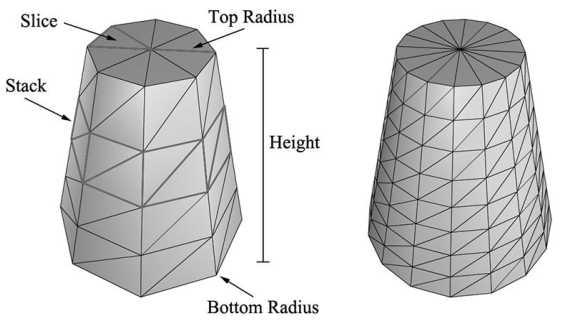
\includegraphics[width=\textwidth]{7-1}
    \centering
    \caption{在此图中,左侧的圆柱体有八个切片和四个堆叠,右侧的圆柱体有十六个切片和八个堆叠。 切片和堆栈控制三角形密度。 请注意,顶部和底部半径可以不同,以便我们可以创建锥形对象,而不仅仅是“纯”圆柱体。}
    \label{fig:7-1}
\end{figure}

%---- 7.4.1.1 ----
\subsubsection{圆柱体边缘几何(Cylinder Side Geometry)}
TODO